\pagestyle{fancy}

\graphicspath{ {Figures/Chapter2_BeamInstrumentation/} }

Beam diagnostics and instrumentation are essential constituents of any particle accelerator. They allow us to monitor the behavior and properties of the particle beam. Without adequate diagnostics, one would be blindly operating an accelerator and it would be impossible to assess problems and improve performances. Different accelerator types require different diagnostics. Similarly, different beam properties require very different instrumentation systems and techniques.  \parencite*[][]{ref:BeamInstrumentationBook}, \parencite*[][]{ref:NotesBeamInst} and \parencite*[][]{ref:CASbeamInst}, are very recommendable references, where the topic of beam instrumentation is covered extensively but yet with a very accessible approach. 

This chapter will focus on describing the principles of some commonly used devices that will be of great relevance for understanding the concepts of this work. We shall focus on the measurements of two beam properties: 

\begin{itemize}
    \item Transverse Beam Profile Measurements: They allow the measurement of the transverse distribution of the particles throughout the accelerator. This measurement is important to control the beam width and position, as well as the transverse matching between different parts of the accelerator facility. In particular, we will focus on Secondary Emission Grids (SEM Grids) and Wire Scanners. 
    \item Beam Intensity Measurements: They allow to measure the total electrical current of the beam, which is one of the most important parameters for the operation of a particle accelerator. Current measurements allow, for example, to determine the transfer efficiencies in linacs and transfer lines. In this case, we will talk about Beam Current Transformers (BCT) and Faraday Cups (FC).
\end{itemize}

\section{Seconday Emission Grids (SEM Grids)}
\label{sec:SEMgrids}

Wire Grids or Secondary Electron EMission grids (SEM Grid) are devices composed of a large number of parallel fixed wires or strips. Figure \ref{fig:SEMgrid} shows an example of a SEM grid detector. They are interceptive devices, during the measurements, each one of the wires interacts directly with the beam of particles. During this process a current, proportional to the number of particles, is generated in each wire.  By measuring the current in all the wires a beam profile can be reconstructed. More detailed explanations about the current generation process and the profile reconstruction will be given in Chapters \ref{ch:BeamMatterInter} and \ref{ch:CurrentModeling}.

\begin{figure}[h]
    \centering
    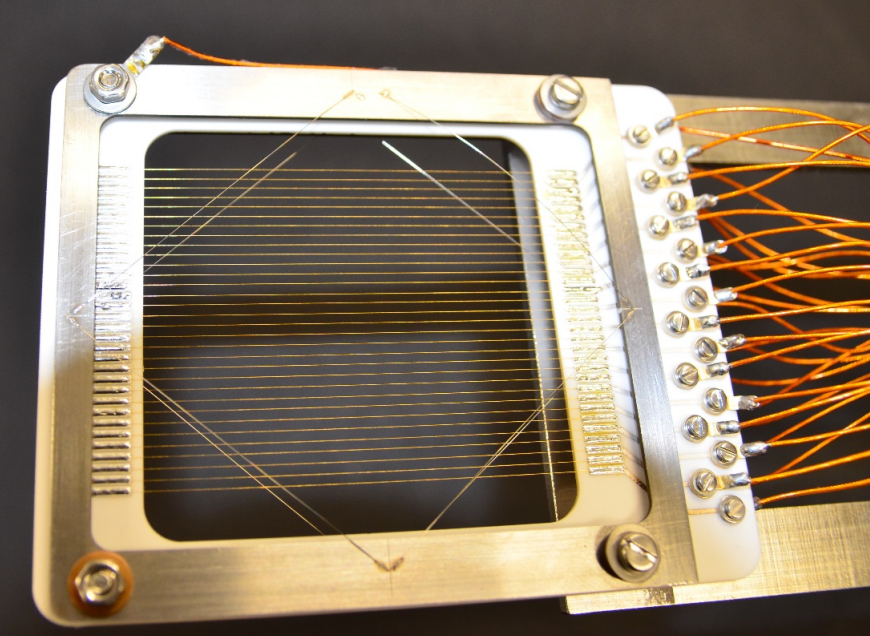
\includegraphics[width=0.6\columnwidth]{SEMGrid/semgrid.png}
    \caption{Example of a SEM grid installed at CERN accelerator Complex. }
    \label{fig:SEMgrid}
\end{figure}

SEM grids allow for a single-shot acquisition, and in some cases, it is possible to observe the evolution of the beam profile in the same pulse. The number of wires and the spacing between them varies from system to system. It is important for the detector to cover the whole range of the beam size and to have enough resolution to properly reconstruct the beam profile. Theoretically, a bigger detector with a larger number of wires would be more convenient. However, a system with too many wires implies an overly complicated acquisition system, it increases the probability of wire cross-talk and augments the construction costs. 

A typical number of wires ranges from 16 to 48. In some devices, the wires are spaced unevenly, with a denser distribution in the center. The diameter-to-spacing of the wires determines the attenuation of the beam current, which becomes an important parameter to consider for particles at low energies as they are fully stopped in the detector's material. It is common to consider that a $10 \%$ of the beam area is covered with the wires. 

The wire materials are selected to optimize signal generation and ensure proper thermal performance. Typical materials used for wire grid designs are Tungsten, Carbon (Graphite, CNT) or Titanium. The motion control of SEM grids is relatively simple, they are either fully inserted or fully retracted, and sometimes they might even be permanently positioned in the beam pipe with no motion control at all. 


\begin{figure}[h]
    \centering
    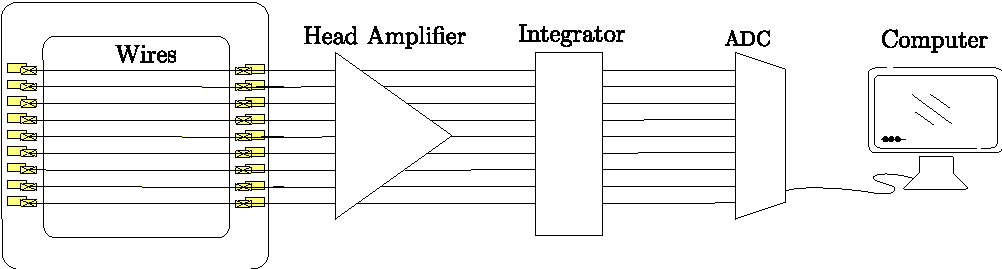
\includegraphics[width=1.0\columnwidth]{SEMgridDataADq/SEMdataAdc.pdf}
    \caption{Schematic representation of SEM Grid Adquisition system. }
    \label{fig:SEMGridReadOutSystem}
\end{figure}

Typically, the data acquisition chain is composed of a head amplifier that sits as near as possible to the grid, often in an area with radiation. It is followed by an integrator or signal conditioning circuit that sits away in a safe room. From the integrator, the signal is fed to a computer controller ADC. This scheme requires one signal cable per wire over the distance from the device to the ADC. 

The main drawbacks of this diagnostics device are the limit on the spatial resolution (which can be hardly reduced to less than a few hundred micrometers), the small wire signals and the complicated data adquisition system. 

\section{Wire Scanners}
\label{sec:WireScan}

Instead of using several wires with individual, expensive electronics, the Wire Scanners consist of a single wire that can be swept through the beam pipe (See figure \ref{fig:WireScan}). The main advantage of this technique is the high resolution that can be accomplished (sub-mm range). It is often used in accelerators with small beam sizes. These devices also intercept the beam of particles, however, its effect is practically negligible.

\begin{figure}[h]
    \centering
    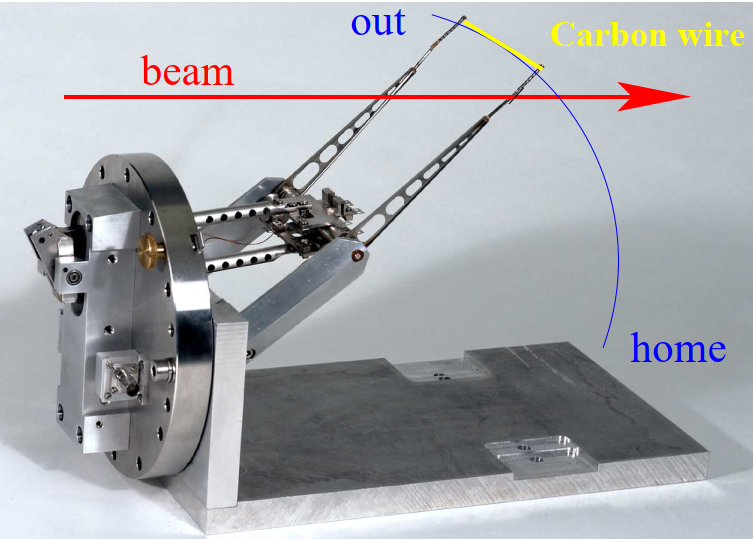
\includegraphics[width=0.6\columnwidth]{WireScanner/WireScanner.png}
    \caption{Rotational Fast Wire Scanner, used at CERN SPS. }
    \label{fig:WireScan}
\end{figure}

In the context of this thesis, we differentiate between two types of wire scanners:

\begin{enumerate}
    \item Slow Wire Scanners: They are commonly used on LINACs or transfer lines. Where the beam energy of the particle beam is small and the pulse structure consists of short pulses and low repetition rates. In this case, the profile is reconstructed by using the current generated in the detector by its interaction with the beam of particles. This signal is typically small and requires careful care in the acquisition. Usually, due to the low repetition rate of the beam in those areas, one sample is taken on each beam pulse, leaving plenty of time to move the wire from one pulse to the rest. 
    \item Fast Wire Scanners: For high energy and high repetition range beams, the profile is reconstructed by measuring a shower of secondary particles generated during the beam/wire interaction. These secondary particles might be hadrons (for proton/heavy ion accelerators) or photons (for electrons accelerators).  The secondary shower is detected outside the beam pipe, with a photo-multiplier tube. The speed of the wire movement varies over a very large range that can go from 1 \si[]{\metre /\second} up to 20 \si[]{\meter /\second}. In this case, the signal measured is typically quite large, due to the high photomultiplier range.  
\end{enumerate}

In both cases, the measurement of the wire position is a crucial aspect of the measurement, as the beam profile is reconstructed by correlating the wire position with the generated signal. The precision of the measurements of the wire scanner positions will therefore be a crucial factor in the measurement precision and resolution. In the case of fast wire scanners, the deformations or vibrations in the wire can also restrict the spatial resolution. Beam position and beam size variations during the measurement period can induce additional errors. 

For both, slow and fast wire scanners, the dimensions of the wire have a direct impact on the signal strengths and the measurement accuracy. In general beam sizes between 10 \si[]{\micro \metre} to 50 \si[]{\micro \metre}  are used.

\section{Beam Current Transformer (BCT)}
\label{sec:BCT}

An electric current flowing through a conductor gives rise to a magnetic field around the conductor, and passing a conducting loop through a magnetic field induces a current through the loop. These well-known principles of induction are used in the Beam Current Transformer (BCT). In this case, the particle beam is the primary current and can be described as: 

\begin{equation}
    I_{beam} = \frac{q e N_{part}}{t}
\end{equation}

Where $N_{part}$ is the number of particles of charge $q$ per unit time $t$. $e$ is the electron charge. This beam current generates a magnetic field as it travels through the accelerator. This magnetic field can be measured by placing a torus with high permeability around the beam. Some windings are placed around the tourus and then connected to an electrical circuit for read-out. Figure \ref{fig:BCTschema} shows a schematic representation of a BCT design. Measuring small beam currents becomes very challenging with these devices.

\begin{figure}[h]
    \centering
    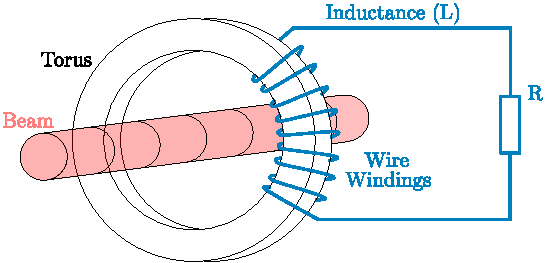
\includegraphics[width=0.6\columnwidth]{BCTschema/BCTschema.pdf}
    \caption{Schema of a current transformer built as a ring-core (torus). }
    \label{fig:BCTschema}
\end{figure}

\section{Faraday Cup (FC)}
\label{sec:FC}

A faraday cup (FC) is a beam stopper that measures the electrical current of the beam. A basic cup design is shown in figure \ref{fig:FaradayCup}. With a Faraday cup, a much lower current can be measured compared to a BCT, of the order of the \si[]{\pico \ampere} for low noise systems. These devices consist of an isolated metal cup connected to a current-sensitive pre amplifier. The current in these detectors is generated by measuring the total charge from the beam of particles that is deposited in them. High energetic particles not depositing all their energy in the detector material can affect negatively the measurement results. Similarly, a Secondary Electron (SE) suppression system has to be included in these devices to avoid errors in the current measurements. This is done by creating very long cups, high voltage suppression close to the entrance or by using a magnetic field. 

\begin{figure}[h]
    \centering
    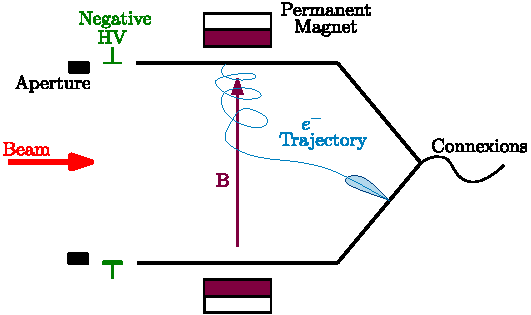
\includegraphics[width=0.6\columnwidth]{FCschema/FCschema.pdf}
    \caption{Schematic Representation of Faraday Cup. }
    \label{fig:FaradayCup}
\end{figure}

Sometimes, Faraday cups are also used for higher beam currents, where measurements with BCTs are also possible as they are easier to implement. In addition, cups serve as beam dumps. For high beam energies, one has to be concerned about the high thermal and structural shocks that these devices might suffer.

\section{Beam Intensity and Profile Measurements at CERN LINAC4.}

In this section, we will briefly show how the instruments just presented are used at CERN, LINAC4. All the results presented in this section correspond to the first profile and current measurements for the LBE run, which took place in November 2019 \parencite*[][]{ref:PresentationLBERun}. The objective of these measurements was to study the transverse profile evolution of the particle beam along the LINAC4 accelerator. 

Figure \ref{fig:Linac4Layout} shows a schematic representation of LINAC4 with the different detectors and locations. In this figure, the yellow circles represent the BCTs. The blue and red rectangles indicate the positions of SEM grids and Wire scanners respectively. Green rectangles indicate positions where SEM grid and Wire scanners are installed at the same position. As we can see from this figure, both BCTs and Beam profile instruments are placed all along LINAC4 so the beam parameters can be measured in all the acceleration stages. 

\begin{figure}[h]
    \centering
    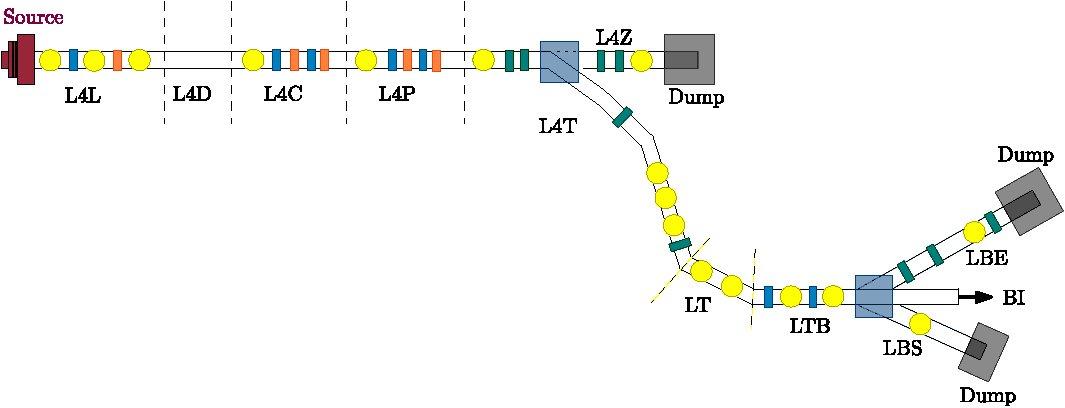
\includegraphics[width=1.0\columnwidth]{Linac4Instrumetnation/Linac4Instruments.pdf}
    \caption{Schematic representation of LINAC4 with the location of some diagnostics devices.}
    \label{fig:Linac4Layout}
\end{figure}

Figure \ref{fig:BCTwithTime} shows an example of intensity measurement taken by the first BCT in the L4T segment. From this figure, one can identify the beam pulse, we can observe that due to the accelerator of $H^{-}$ particles at LINAC4, the registered current is negative. In this case, the beam pulse length was 36 \si[]{\micro \second} with an average intensity of $\sim 17 $ \si[]{\milli \ampere}. One can observe the 1 \si[]{\micro \second} gaps generated by the chopper, which make the beam pulse ready to be injected into the different pulse rings. 

\begin{figure}
    \centering
    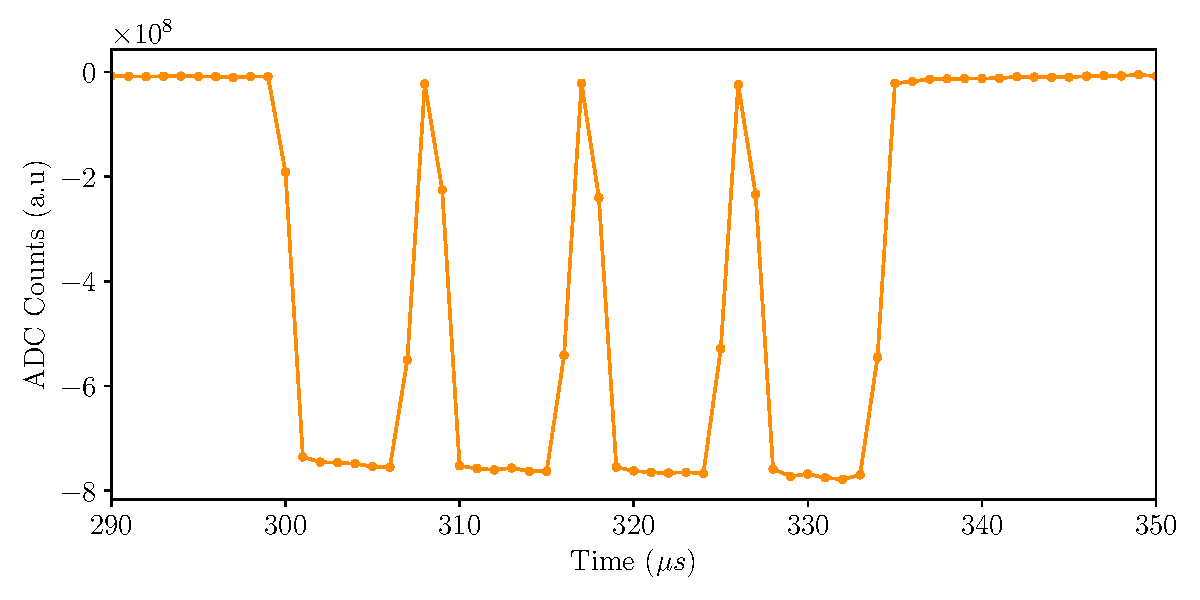
\includegraphics[width=0.7\columnwidth]{IntensityVStime/IntensityVStime.pdf}
    \caption[The LOF caption]{Beam current shape along beam pulse, from first BCT in L4T line.}
    \label{fig:BCTwithTime}
\end{figure}

By measuring the average current of the beam at all the available BCTs, one can assess the beam transmission along the accelerator. Figure \ref{fig:BeamTrans} shows an example of beam transmission measured along the accelerator. From this figure one can observe how in all parts of the accelerator, except for the first two BCTs in the L4L line, the current remains quite constant around $\sim 17$ \si[]{\milli \ampere}.  Similarly, the beam transmission remains very close to $100 \%$ along the whole accelerator. 

\begin{figure}
    \centering
    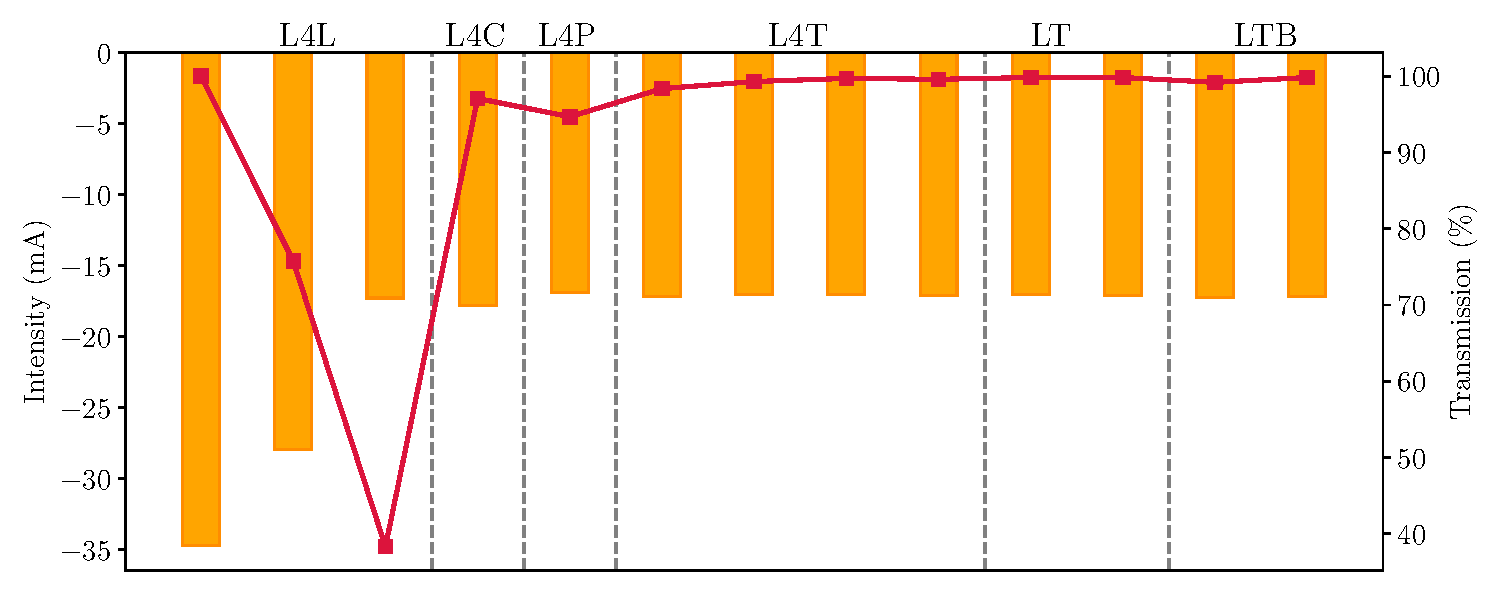
\includegraphics[width=0.9\columnwidth]{BCT_Transmission/TransmissionBCT.pdf}
    \caption{Average intensity measured by the different BCTs at LINAC4. Transmission along the LBE line.}
    \label{fig:BeamTrans}
\end{figure}


Similarly, the beam profile was measured along the accelerator, to cross-check the beam evolution as well as to assess the integrity and status of the devices installed along the accelerator.  Figure \ref{fig:HorizontalProf} shows the measurements of the horizontal profile of the beam along the LINAC4 accelerator. All these measurements were taken with the SEM grids. From this figure we can observe:

\begin{figure}
    \centering
    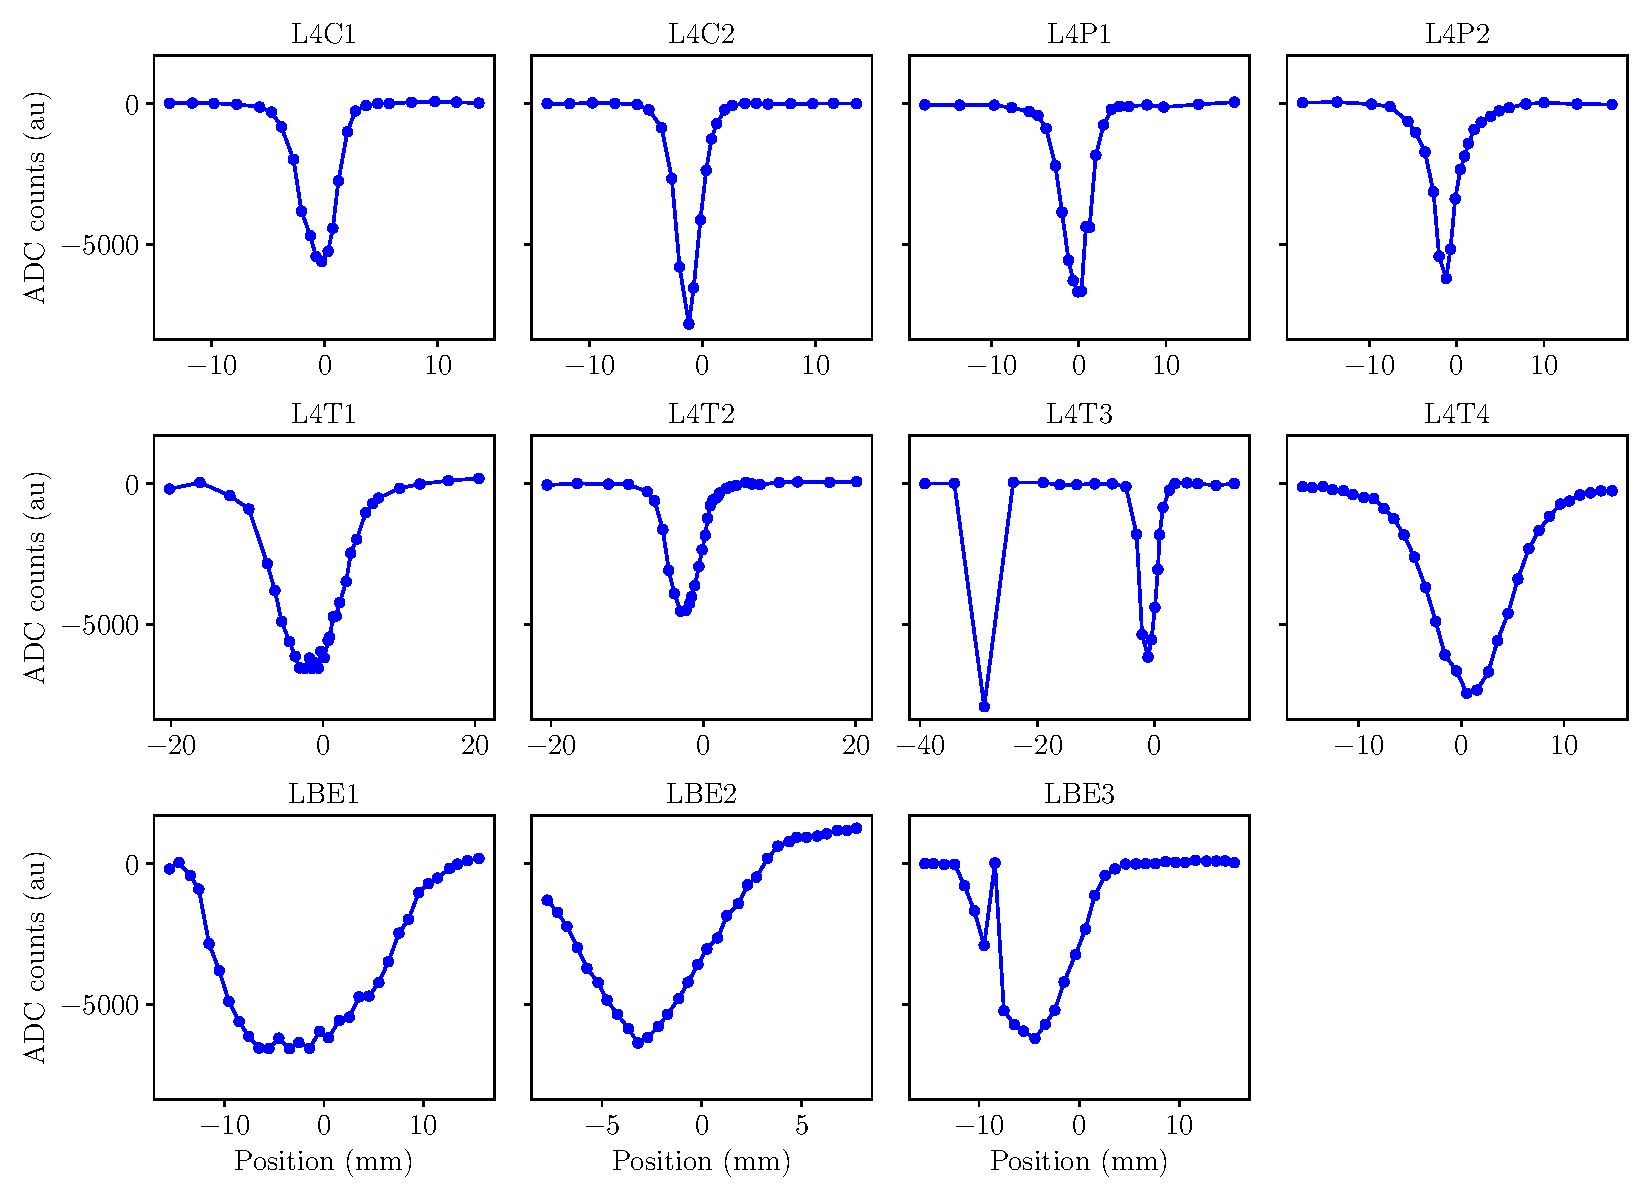
\includegraphics[width=1.0\columnwidth]{SigmaEvol/HorEvol.pdf}
    \caption{Horizontal transversal beam profile measured by the differt detectors at LINAC4}
    \label{fig:HorizontalProf}
\end{figure}

\begin{itemize}
    \item The beam profile seemed to be very much gaussian in all the measurement points except for LBE1 and LBE2 positions.
    \item Broken wires: SEM grids L4T2 and LBE3 present a broken wire that must be repaired. Wires 12-13 and 14-15 in L4P1 are glued together. 
    \item L4T1 and LBE1 present strange strange oscillations in the wires measuring the highest intensities. 
    \item Some of the grids have an even wire separation while others present a noneven wire distancing. Due to the beam not always being centered having smaller wire separation at the center of the grid des not seem to be that helpful.
    \item Not depicted, however, the data acquisition system for the detectors in the LBE sector had to be corrected to properly acquire the data.
\end{itemize}




Here we presented only the evolution of the horizontal profile, however, the evolution of the vertical profile was similarly studied. In the case of the vertical profile, a non-gaussian beam was observed in some of the locations. Figure \ref{fig:VertProf} shows an example of a vertical profile taken with both the second SEM grid and the second Wire Scanner from the L4T line. In this case, the particle beam clearly shows some shoulders or tails that push it away from the gaussian distribution. Another thing that one can observe from this figure, is the great agreement between the beam profile measurements by the sem grid and the wire scanner. 


These measurements were the first systematic set of measurements of the LBE run, they helped understand the beam evolution along the accelerator and thus helped correct the observed irregularities. These measurements also helped assess and correct any issue on the measuring devices, such as broken wires, position misreadings, data acquisition problems, etc.  

\begin{figure}[h]
    \centering
    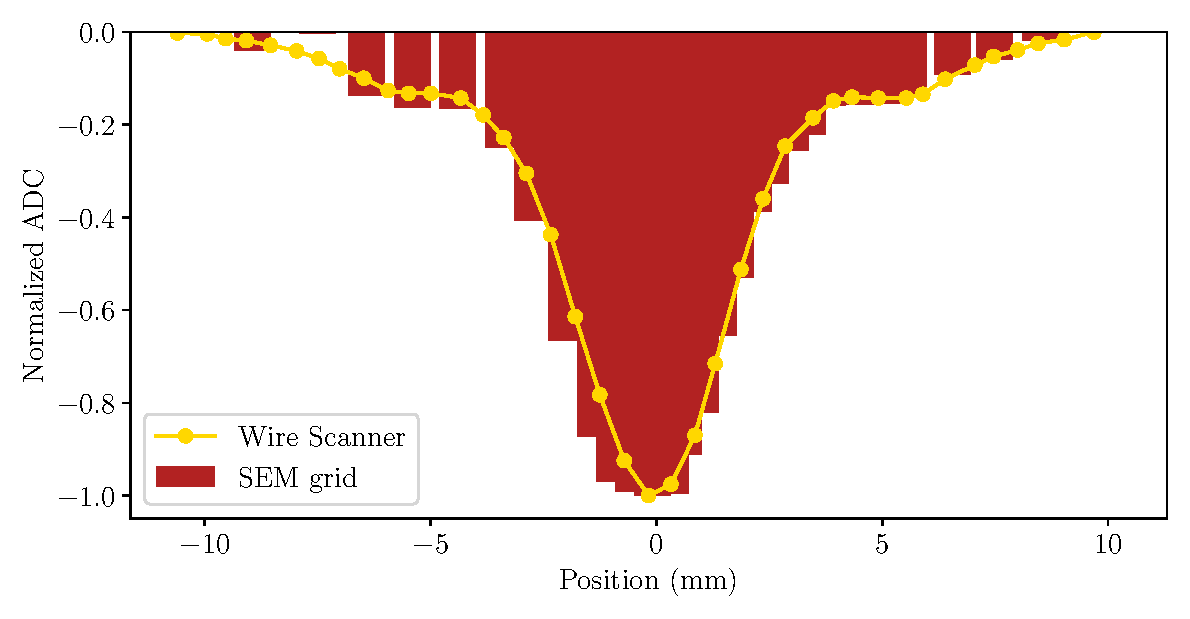
\includegraphics[width=0.6\columnwidth]{VertProf/VertProf.pdf}
    \caption{Vertical transverse profile measured by the second SEM grid and second wire scanner of the L4T line at Linac4.}
    \label{fig:VertProf}
\end{figure}




